
\newcommand{\obj}{o}
\newcommand{\off}{w}


%%%%self define math symbol
\def \eg{{\em e.g.,}}
\def \ie{{\em i.e.,}}
\def \etc{{\em etc.}}
\def \mm{{\em mm}}
\def \cm{{\em cm}}
\def \m{{\em m}}
\def \one{{\em i)}}
\def \two{{\em ii)}}
\def \three{{\em iii)}}
\def \four{{\em iv)}}

\def \Safe{\mathrm{S}}
\def \Robust{\mathrm{R}}


\section{Robustness Verification via Reachability Analysis}\label{chap:reachabilityAnalysis}

As discussed in previous chapters, concerns have been raised about the suitability of deep neural networks (DNNs), or systems with DNN components, for deployment in safety-critical applications. 
%To ease this concern and gain users' trust, DNNs need to be certified similarly to %software and hardware  systems such as airplanes and automobiles. 
%
To this end, besides those aforementioned verification techniques, we can also study a generic reachability problem in which, for a given DNN, an input subspace and a function over the network's outputs, computes the upper and lower bounds over the values of the function. The function is generic, with the only requirement that it is Lipschitz continuous. %and has the DNN's output as its input. 
We argue that this problem is fundamental for the certification of DNNs, %can be a core problem towards certifying DNNs 
as it can be instantiated into several key correctness problems, including adversarial example generation \cite{szegedy2014intriguing,DBLP:journals/corr/GoodfellowSS14}, safety verification \cite{HKWW2017,katz2017reluplex,RWSHKK201  8}, and output range analysis \cite{LM2017,dutta2017output}.

%$R_j(X')$ for a given class label $j\in [1..m]$.
% is the set of possible confidence levels $c_j(x)$ over the label $j$. 
% An error bound may be needed for practical reasons. 

To certify a system, a certification approach needs to provide not only a result but also a guarantee over the result, such as the error bounds. 
Existing approaches for analysing DNNs with provable guarantees work by either reducing the problem to a constraint satisfaction problem that can be solved by MILP \cite{LM2017,CNR2017,bunel2017piecewise,xiang2017output}, SAT \cite{NKPSW2017} or SMT \cite{katz2017reluplex,bunel2017piecewise} solvers, or applying search algorithms over discretised vector spaces \cite{HKWW2017,wicker2018feature}. Even though they are able to achieve guarantees, they suffer from two major weaknesses. Firstly, their subjects of study are restricted. 
More specifically, they can only work with layers conducting linear transformations (such as convolutional and fully-connected layers) and simple non-linear transformations (such as ReLU). They cannot work with other important layers, such as the Sigmoid, Max pooling and Softmax layers that are widely used in state-of-the-art networks. Secondly, the scalability of the constraint-based approaches is significantly limited by both the capability of the solvers and the size of the network. However, state-of-the-art networks usually have millions or even billions of hidden neurons. 

This chapter will introduce a novel approach to tackle the generic reachability problem, which does not suffer from the above weaknesses and provides provable guarantees %over its results 
in terms of the upper and lower bounds over the errors. The approach is inspired by recent advances made in the area of global optimisation~\cite{gergel2016adaptive,grishagin2018convergence}. 
For the input subspace defined over a set of input dimensions, an adaptive nested optimisation algorithm is developed. The performance of this algorithm is not dependent on the size of the network, and it can therefore scale to work with large networks. 

This algorithm assumes certain knowledge about the DNN. However, instead of directly translating the activation functions and their parameters (i.e., weights and bias) into linear constraints, % as done in the reduction approaches, 
it needs a Lipschitz constant of the network. For this, we show that several layers that cannot be directly translated into linear constraints are actually Lipschitz continuous, and we can compute a Lipschitz constant by analysing the activation functions and their parameters. This method is implemented as a software tool DeepGO\footnote{It is available on \url{https://github.com/trustAI/DeepGO}.}. 
%and evaluate its performance by comparing with existing constraint-based approaches, namely, SHERLOCK \cite{dutta2017output} and Reluplex \cite{katz2017reluplex}. We also demonstrate % on several problems that can be handled by them. Our experiments include those networks that cannot be handled by existing algorithms. 
% our tool on DNNs that are beyond the capability of existing tools.

%Practically, the layer-to-layer mapping functions can be various types of activation functions such as ReLU, Leaky ReLU, sigmoid function, Hyperbolic tangent function etc., or different pooling operations such as max pooling and contrast-normalization pooling, and softmax layer (usually in the last layer). Noted that existing methods of reachability analysis for DNNs are all based on MLP [?], SAT [?] or SMT [?] techniques, which enable them has the following three major limitations: \one~they are only workable on the ReLU activation functions due to the linearizion formulation; \two~they cannot analyses softmax layer which enables their reachability analysis not complete; and \three~those methods are based on a layer-by-layer analysis which makes them only workable for a small-scale neural network(such as 3-layer NN with only hundreds of neurons. 

%To deal with the above limitation, in this paper, we tackle the problem from a "black-box" point of view, which is neither depends on the layer-by-layer analysis nor built upon any MLP solvers. The only assumption we rely on is that the targeted deep neural network satisfies the Lipschitz continuity assumption.
		%\vspace{1mm}

%\vspace{-3pt}

\subsection{Lipschitz Continuity of Deep Learning}\label{sec:lipschitz}

This section shows that feed-forward DNNs are Lipschitz continuous.
Let $f: \mathbb{R}^n \rightarrow \mathbb{R}^m$ be a $N$-layer 
%feed-forward neural 
network such that, for a given input $\mathbf{x}\in \mathbb{R}^n$, $f(\mathbf{x}) = \{c_1,c_2,...,c_m\}\in \mathbb{R}^m$ represents the confidence values for $m$ classification labels. Specifically, we have 
$f(\mathbf{x}) = f_N(f_{N-1}(...f_1(\mathbf{x};\mathbf{W}_1,\mathbf{b}_1);\mathbf{W}_2,\mathbf{b}_2);...);\mathbf{W}_N,\mathbf{b}_N)
$ where $\mathbf{W}_i$ and $\mathbf{b}_i$ for $i = 1,2,...,N$ are learnable parameters and $f_i(\mathbf{z}_{i-1};\mathbf{W}_{i-1},\mathbf{b}_{i-1})$ is the function mapping from the output of layer $i-1$ to the output of layer $i$ such that $\mathbf{z}_{i-1}$ is the output of layer $i-1$. Without loss of generality, we normalise the input $\mathbf{x}\in [0,1]^n$. The output $f(\mathbf{x})$ is usually normalised to be in $[0,1]^m$ with a Softmax layer. 
	


\begin{definition}[Lipschitz Continuity]
	Given two metric spaces $(\mathbf{X}, d_\mathbf{X})$ and $(\mathbf{Y}, d_\mathbf{Y})$, where $d_\mathbf{X}$ and $d_\mathbf{Y}$ are the metrics on the sets $\mathbf{X}$ and $\mathbf{Y}$ respectively, a function $f: \mathbf{X}\rightarrow \mathbf{Y}$ is called {\em Lipschitz continuous} if there exists a real constant $K\geq0$ such that, for all $\mathbf{x}_1, \mathbf{x}_2 \in \mathbf{X}$:
	\begin{equation}
	 d_\mathbf{Y}(f(\mathbf{x}_1), f(\mathbf{x}_2)) \le K d_\mathbf{X}(\mathbf{x}_1, \mathbf{x}_2).
	\end{equation}
	$K$ is called the {\em Lipschitz constant} for the function $f$. The smallest $K$ is called {\em the Best Lipschitz constant}, denoted as $K_{best}$.
\end{definition}

The work in \cite{szegedy2014intriguing} shows that deep neural networks with half-rectified layers (\ie~convolutional or fully connected layers with ReLU activation functions), max pooling and contrast-normalization layers are Lipschitz continuous. They prove that the upper bound of the Lipschitz constant can be estimated via the operator norm of learned parameters $\mathbf{W}$. Furthermore, other researchers theoretically demonstrate that the Softmax layer, Sigmoid and Hyperbolic tangent activation functions also satisfy the Lipschitz continuity, the details of the proof can be found in the work of \cite{RHK2018}.

% First we need the following lemma~\cite{sohrab2003basic}.

% \begin{mylemma}\label{theo-1}
% Let $f: \mathbb{R}^n \rightarrow \mathbb{R}^m$,	if $||\partial{f(\mathbf{x})}/\partial{\mathbf{x}}|| \leq K$ for all $\mathbf{x} \in [\mathbf{a}, \mathbf{b}]^n$, then $f$ is Lipschitz continuous on $[\mathbf{a}, \mathbf{b}]^n$ and $K$ is its Lipschitz constant, where $||*||$ represents a norm operator.
% \end{mylemma}

% Based on this lemma, we have the following theorem.

% \begin{theorem}
% Convolutional or fully connected layers with the sigmoid activation function $s(W\mathbf{x}+b)$, Hyperbolic tangent activation function $t(W\mathbf{x}+b)$, and softmax function $p(\mathbf{x})_j$ are Lipschitz continuous and their Lipschitz constants are $\dfrac{1}{2}\norm{W}$, $\norm{W}$, and $\sup_{i,j}(\norm{\mathbf{x}_i} + \norm{\mathbf{x}_i\mathbf{x}_j})$, respectively.
% \end{theorem}

% \begin{myproof}
% First of all, we show that the norm operators of their Jacobian matrices are bounded.

% (1)~Layer with sigmoid activation $s(q) = 1/(1+e^{-q})$ with $ q = W\mathbf{x}+b$:
% \begin{equation}
% \begin{split}
% \norm{\dfrac{\partial{s(\mathbf{x})}}{\partial{\mathbf{x}}}} = \norm{\dfrac{\partial{s(q)}}{\partial{q}} \dfrac{\partial{q}}{\partial{\mathbf{x}}}}
% \leq \norm{\dfrac{\partial{s(q)}}{\partial{q}}} \norm{\dfrac{\partial{q}}{\partial{\mathbf{x}}}}\\
% \leq \norm{s(q)\circ(\mathbf{1}-s(q))}\norm{W}\leq \dfrac{1}{4}\norm{W}
% \end{split}
% \end{equation}

% (2)~Layer with Hyperbolic tangent activation function $t(q) = 2/(1+e^{-2q})-1$ with $ q = W\mathbf{x}+b$:
% \begin{equation}
% \begin{split}
% \norm{\dfrac{\partial{t(\mathbf{x})}}{\partial{\mathbf{x}}}} = \norm{\dfrac{\partial{t(q)}}{\partial{q}} \dfrac{\partial{q}}{\partial{\mathbf{x}}}}
% \leq \norm{\dfrac{\partial{t(q)}}{\partial{q}}} \norm{\dfrac{\partial{q}}{\partial{\mathbf{x}}}}\\
% \leq \norm{\mathbf{1}-t(q)\circ t(q))}\norm{W}\leq \norm{W}
% \end{split}
% \end{equation}

% (3)~Layer with softmax function $p(\mathbf{x})_j = e^{\mathbf{x}_j}/(\sum_{k = 1}^{n}{e^{\mathbf{x}_k}})$ for $j = 1,...,m$ and $n = m$ (dimensions of input and output of softmax are the same):
% \begin{equation}
% \begin{split}
% \norm{\dfrac{\partial{p(\mathbf{x})_j}}{\partial{\mathbf{x}_i}}} = 
% \left\{
% \begin{array}{ll}
% \mathbf{x}_i(1-\mathbf{x}_j), ~~i = j\\
% -\mathbf{x}_i\mathbf{x}_j,~~i\ne j
% \end{array}
% \right. \leq \sup_{i,j} (\norm{\mathbf{x}_i} + \norm{\mathbf{x}_ix_j})
% \end{split}
% \end{equation}
% Since the softmax layer is the last layer of a deep neural network, we can estimate its supremum based on Lipschitz constants of previous layers and box constraints of DNN's input.

% The final conclusion follows by Lemma 1 and the fact that all the layer functions are bounded on their Jacobian matrix. 
% \end{myproof}


\subsection{Reachability Analysis of Deep Learning}

In this section, we present the formulate the problem of confidence reachability of a neural network. 
Let $\obj: [0,1]^m \rightarrow \mathbb{R}$ be a Lipschitz continuous function statistically evaluating the outputs of the network. Our problem is to find its upper and lower bounds given the set $\mathbf{X}'$ of inputs to the network. Because both the network $f$ and the %statistical evaluation 
function $\obj$ are Lipschitz continuous, all values between the upper and lower bounds have a corresponding input, i.e., are reachable. 

\begin{definition}[Reachability of Neural Network]
Let $\mathbf{X}'\subseteq [0,1]^n$ be an input subspace and $f: \mathbb{R}^n \rightarrow \mathbb{R}^m$ a network.
% such that $f(x) = \{c_1,...,c_j,...,c_m\}\in [0,1]^m$ and $c_j$ is the $j$-th confidence output representing the probability of input $x$ belonging to $j$-th classification label. We also use $c_j(x)$ to represent the $j$-th output of DNN given input $x$. Then 
The reachability of $f$ over the function $\obj$ under an error tolerance $\epsilon \geq 0$ is a set $R(\obj,\mathbf{X}',\epsilon) = [l,u]$ such that 
\begin{equation}
\begin{split}
\inf_{\mathbf{x}' \in \mathbf{X}'} \obj(f(\mathbf{x}')) -\epsilon \leq l \leq \inf_{\mathbf{x}' \in \mathbf{X}'} \obj(f(\mathbf{x}')) +\epsilon \\
\sup_{\mathbf{x}' \in \mathbf{X}'} \obj(f(\mathbf{x}')) - \epsilon \leq u \leq \sup_{\mathbf{x}' \in \mathbf{X}'} \obj(f(\mathbf{x}')) + \epsilon.
\end{split}
\end{equation}
We write $u(\obj,\mathbf{X}',\epsilon)=u$ and $l(\obj,\mathbf{X}',\epsilon)=l$ for the upper and lower bound, respectively. 
%Confidence Upper Bound (CUB) and Confidence Lower Bound (CLB), respectively. 
Then the reachability diameter is 
	\begin{equation}
           D(\obj,\mathbf{X}',\epsilon) =u(\obj,\mathbf{X}',\epsilon)-l(\obj,\mathbf{x}',\epsilon).
	\end{equation}
Assuming these notations, we may write $D(\obj,\mathbf{X}',\epsilon;f)$ if we need to explicitly refer to the network $f$. 
\end{definition}

In the following, we instantiate $\obj$ with a few concrete functions, and show that several key verification problems for DNNs can be reduced to our reachability problem. 

\begin{definition}[Output Range Analysis]
Given a class label $j\in [1,..,m]$, we let $\obj = \Pi_j$ such that $\Pi_j((c_1,...,c_m))=c_j$. 
\end{definition}

We write $c_j(\mathbf{x}) = \Pi_j(f(\mathbf{x}))$ for the network's confidence in classifying $\mathbf{x}$ as label $j$. 
Intuitively, output range \cite{dutta2017output} quantifies how a certain output of a deep neural network (\ie~classification probability of a certain label $j$) varies in response to a set of DNN inputs with an error tolerance $\epsilon$. Output range analysis can be easily generalised to logit \footnote{Logit output is the output of the layer before the softmax layer. The study of logit outputs is conducted in, e.g., \cite{dutta2017output}.} range analysis.

We show that the safety verification problem \cite{HKWW2017} can be reduced to solving the reachability problem. 

\begin{definition}[Local Safety]
A network $f$ is safe with respect to an input $\mathbf{x}$ and an input subspace $\mathbf{X}'\subseteq [0,1]^n$ with $\mathbf{x} \in \mathbf{X}'$, written as $\Safe(f,\mathbf{x},\mathbf{X}')$, if 
\begin{equation}
\forall \mathbf{x}' \in \mathbf{X}': \arg\max_{j} c_j(\mathbf{x}') = \arg\max_{j} c_j(\mathbf{x})
\end{equation} 
%where $c_j(x) = f(x)_j$ returns $N$'s confidence in classifying $x$ as label $j$. 
\end{definition}

We have the following reduction theorem. 

%For the reduction, we define two functions $o_1=\Pi_j$ such that $j=\arg\max_{j}c_j(x)$, and $o_2 = +_{-j}$ such that $+_{-j}(c_1,...,c_m) = \sum_{i=1, i\neq j}^{m} c_i$. Therefore, we have 

\begin{theorem}\label{thm:safety}
A network $f$ is safe with respect to $\mathbf{x}$ and $\mathbf{X}'$ s.t. $\mathbf{x} \in \mathbf{X}'$ if and only if
$u(\oplus,\mathbf{X}',\epsilon) \leq 0$,
%$l(\Pi_j,X',\epsilon) \geq u(\oplus_{-j},X',\epsilon)$
where $\oplus(c_1,...,c_m) = \max_{i\in \{1..m\}}(\Pi_{i} (c_1,...,c_m) - \Pi_{j} (c_1,...,c_m))$ and $j=\arg\max_{j}c_j(\mathbf{x})$. The error bound of the safety decision problem by this reduction is $2\epsilon$. 
\end{theorem}

It is not hard to see that the adversarial example generation \cite{szegedy2014intriguing}, which is to find an input $\mathbf{x}' \in \mathbf{X}'$ such that $\arg\max_{j} c_j(\mathbf{x}') \neq \arg\max_{j} c_j(\mathbf{x})$, is the dual problem of the safety problem. 

% The following two problems define the robustness comparisons between the networks and/or the inputs. 

% \begin{definition}[Model Robustness Comparison]
% Given two homogeneous\footnote{Here, two networks are homogeneous if they are applied on the same classification task but may have different network architectures (e.g., layer numbers, layer types, etc) and/or parameters.}
% %E.g., two different neural networks but both are for the MNIST image classification task.} 
% networks $f$ and $g$, we say that model $f$ is strictly more robust than model $g$ with respect to a function $\obj$, an input subspace $\mathbf{X}'$ and an error bound $\epsilon$, written as $\Robust_{o,\mathbf{X}',\epsilon}(f,g)$, if $D(\obj,\mathbf{X}',\epsilon;f) < D(\obj,\mathbf{X}',\epsilon;g)$.

% %$j$-th output and an input subspace $\bar{x}$ if $D_j(\bar{x};f(x)) < D_j(\bar{x};g(x))$.
% \end{definition}

% \begin{definition}[Subspace Robustness Comparison]
% 	Given two input sub-spaces $\mathbf{X}'$ and $\mathbf{X}''$ and a network $f$, we say that $f$ is more robust on subspace $\mathbf{X}'$ than on subspace $\mathbf{X}''$ with respect to a statistical function $\obj$ and an error bound $\epsilon$, written as $\Robust_{f,o,\epsilon}(\mathbf{X}',\mathbf{X}'')$, if $D(\obj,\mathbf{X}',\epsilon) < D(\obj,\mathbf{X}'',\epsilon)$.
% %$D_j(\bar{x}) < D_j(\hat{x})$.
% \end{definition}

Thus, by instantiating the function $\obj$, we can quantify a network's output/logit range and verify whether a network is robust or safe.
		%\vspace{-1mm}

%\vspace{-3pt}
\subsection{Confidence Reachability with Guarantees}
%\vspace{-1pt}

Section~\ref{sec:lipschitz} shows that a deep feedforward neural network is Lipschitz continuous regardless of its layer depth, activation functions and the number of neurons. Now, to solve the reachability problem, we need to find the \emph{global} minimum and maximum values given an input subspace, assuming that we have a Lipschitz constant $K$ for the function $o\!\cdot\!f$. In the following, we let $\off = o\!\cdot\!f$ be the concatenated function. Without loss of generality, we assume the input space $\mathbf{X}'$ is a box-constraint (i.e., measured by $L_\infty$-norm distance), which is clearly feasible since images are usually normalised into $[0,1]^n$ before being fed into a neural network.

% Thus we need to solve the following problem. Here we start to use $x$ instead of $\bar{x}$ (we can treat the fixed dimensions in input space as a learned parameters in neural network) and drop index $j$ (since we can perform the some analysis to each output separately). 
The computation of the minimum value is reduced to solving the following optimisation problem with guaranteed convergence to the global minimum (the maximisation problem can be similarly solved by minimising the negative objective function):
\begin{equation}\label{equ-8}
\begin{split}
\min\limits_{\mathbf{x}}~~\off(\mathbf{x}),~~~s.t.~~\mathbf{x} \in [a,b]^n
\end{split}
\end{equation}
However, the above optimisation is very challenging since $\off(\mathbf{x})$ is a highly non-convex function which cannot be guaranteed to reach the global minimum by regular optimisation schemes based on gradient descent. Inspired by an idea from optimisation, e.g., \cite{piyavskii1972algorithm,TZ1989}, we design another continuous function $h(\mathbf{x},\mathbf{y})$, which serves as a lower bound of the original function $\off(\mathbf{x})$. Specifically, we need 
%This idea is also widely adopted in optimization community.
\begin{equation}\label{equ-9}
\begin{split}
\forall \mathbf{x}, \mathbf{y} \in [a,b]^n,~ h(\mathbf{x},\mathbf{y}) \leq \off(\mathbf{x})~~\text{and}~~h(\mathbf{x},\mathbf{x}) = \off(\mathbf{x})
\end{split}
\end{equation}
%
Furthermore, for $i\geq 0$, we let $\mathcal{Y}_i = \{\mathbf{y}_0,\mathbf{y}_1,...,\mathbf{y}_i\} $ be a finite set containing $i+1$ points from the input space $ [a, b]^n$, and let $\mathcal{Y}_i \subseteq \mathcal{Y}_k$ when $k>i$, then we can define a function
$H(\mathbf{x};\mathcal{Y}_i) = \max_{\mathbf{y}\in \mathcal{Y}_i } h(\mathbf{x},\mathbf{y})$
 which satisfies the following relation:
\begin{equation}
H(\mathbf{x}; \mathcal{Y}_i) < H(\mathbf{x}; \mathcal{Y}_k)\leq %\inf_{x\in [a,b]^n}
\off(\mathbf{x}), \forall i < k
\end{equation}

We use $l_i = \inf_{\mathbf{x}\in [a,b]^n} H(\mathbf{x};\mathcal{Y}_i)$ to denote the minimum value of $H(\mathbf{x};\mathcal{Y}_i)$ for $\mathbf{x}\in [a,b]^n$. Then we have 
%can get the following relation:
\begin{equation}
l_0< l_1< ... < l_{i-1}< l_i \leq \inf_{\mathbf{x}\in [a,b]^n} \off(\mathbf{x})
\end{equation}
Similarly, we need a sequence of upper bounds $u_i$ to have 
\begin{equation}\label{eqn-14}
\begin{split}
l_0< ... < l_i \leq \inf_{\mathbf{x}\in [a,b]^n} \off(\mathbf{x})\leq u_i< ...< u_0
\end{split}
\end{equation}
By Expression (\ref{eqn-14}), we can have the following:
\begin{equation}\label{eqn-15}
\begin{split}
\lim\limits_{i\to \infty}l_i = \min_{\mathbf{x}\in [a,b]^n} \off(\mathbf{x}) \text{   and   }
\lim\limits_{i\to \infty}(u_i - l_i) = 0
\end{split}
\end{equation}

Therefore, we can asymptotically approach the global minimum. Practically, we execute a finite number of iterations by using an error tolerance $\epsilon$ to control the termination. 
%
%\begin{myremarks}
%	Whenever terminated, it returns a lower bound and a upper bound of the global minimum, and we can evaluate the quality of global minimum obtained so far.
%\end{myremarks}
%
In the next section, we present the approach, which constructs a sequence of lower and upper bounds, and show that it can converge with an arbitrarily-small error bound. 
%To handle the high-dimensionality of DNNs, our approach is inspired by the idea of adaptive nested optimisation in \cite{gergel2016adaptive}, with significant differences in the detailed algorithm and convergence proof. 

%We first discuss the one-dimension case and then the multiple-dimension case.
\begin{figure}[t]
	\centering
	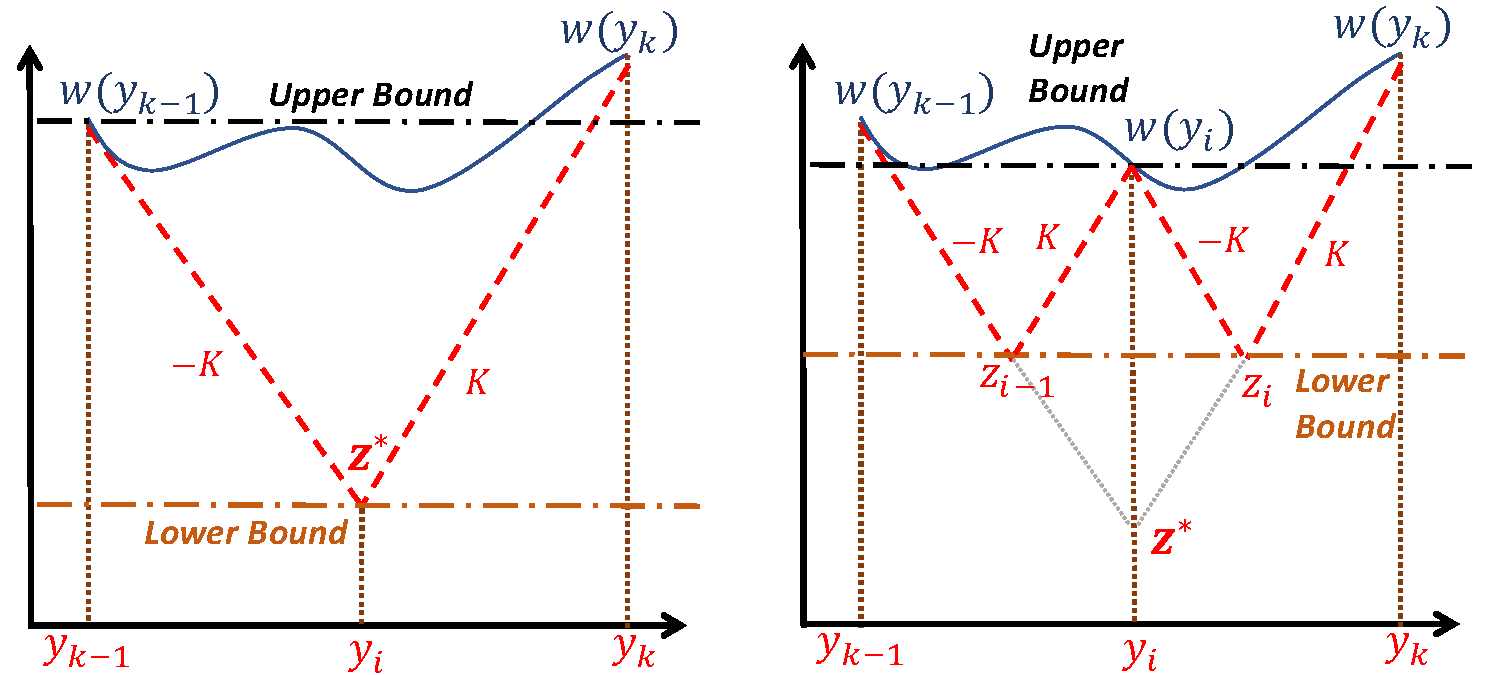
\includegraphics[width=1\linewidth]{images/robustnessVerification/f1.pdf}
	\caption{A lower-bound function designed via Lipschitz constant}
	\label{fig-1}
\end{figure}


\subsubsection{One-dimensional Case}\label{sec:onedimensional}


We first introduce an algorithm which works over one dimension of the input, and therefore is able to handle the case of $x \in [a,b]$ in Eqn.~(\ref{equ-8}).
%, based on Section 2 and Theorem~1, we can estimate the Lipschitz constants of a neural network numerically either or analytically. 
The multi-dimensional optimisation algorithm will be discussed in the next section by repeatedly utilising the one-dimensional algorithm. 
We define the following lower-bound function.
\begin{equation}\label{eqn-10}
\begin{split}
h({x},y) = \off(y) - K|{x}-y| \\
H({x};\mathcal{Y}_i) = \max\limits_{y\in \mathcal{Y}_i }~~\off(y) - K|{x}-y|
\end{split}
\end{equation}
where $K > K_{best}$ is a Lipschitz constant of $\off$ and $H({x};\mathcal{Y}_i)$ intuitively represents the lower-bound saw-tooth function shown as Fig.~\ref{fig-1}.
%$L \geq K_{best}$ and we can estimate by $L = |d(c(x))/dx| + \eta$ $(\eta \geq 0)$ based on Theorem~1. 
The set of points $\mathcal{Y}_i$ is constructed recursively. Assuming that, after $(i-1)$-th iteration, we have $\mathcal{Y}_{i-1} = \{y_0,y_1,..,y_{i-1}\}$, whose elements are in ascending order, and sets 
$$
\off(\mathcal{Y}_{i-1} )=\{\off(y_0), \off(y_1),..,\off(y_{i-1})\}
$$
$$\mathcal{L}_{i-1} = \{l_0,l_1,...,l_{i-1}\}$$
$$\mathcal{U}_{i-1} = \{u_0,u_1,...,u_{i-1}\}$$
$$\mathcal{Z}_{i-1} = \{z_1,...,z_{i-1}\}$$
%where $z_{k} = \dfrac{\off(y_{k})+ \off(y_{k-1})}{2} - \dfrac{K(y_{k} - y_{k-1})}{2}, \forall k = 1,2,..,i-1$. 
%
The elements in sets $\off(\mathcal{Y}_{i-1} )$, $\mathcal{L}_{i-1}$ and $\mathcal{U}_{i-1}$ have been defined earlier. The set $\mathcal{Z}_{i-1}$ records the smallest values $z_k$ computed in an interval $[y_{k-1},y_k]$.

In $i$-th iteration, we do the following sequentially:
\begin{itemize}

%\item Numerically estimate Lipschitz constant as $K = \eta \max_{j = 1,...,i-1} \{(\off(y_j) - \off(y_{j-1}))/(y_j - y_{j-1})\}$ where $\eta > 1$.

	\item Compute $y_i = \arg\inf_{{x}\in [a,b]} H({x};\mathcal{Y}_{i-1})$ as follows. Let $z^* = \min{\mathcal{Z}_{i-1} }$ and $k$ be the index of the interval $[y_{k-1},y_k]$ where $z^*$ is computed. Then we let 
\begin{equation}\label{equ:newpoint}
y_i = \dfrac{y_{k-1}+y_k}{2} - \dfrac{\off(y_{k}) - \off(y_{k-1})}{2K}
\end{equation}

 and have that $y_i \in (y_{k-1},y_k)$. 
	
	\item Let $\mathcal{Y}_i = \mathcal{Y}_{i-1}\cup\{y_i\}$, then reorder $\mathcal{Y}_i$ in ascending order, and update $\off(\mathcal{Y}_{i} )=\off(\mathcal{Y}_{i-1})\cup \{\off(y_i)\}$.
	
	\item Calculate 
	\begin{equation}\label{eqn-16}
	z_{i-1} = \dfrac{\off(y_{i})+ \off(y_{k-1})}{2} - \dfrac{K(y_{i} - y_{k-1})}{2}\end{equation}
	
	\begin{equation}\label{eqn-17}
	z_{i} = \dfrac{\off(y_{k})+ \off(y_{i})}{2} - \dfrac{K(y_{k} - y_{i})}{2}\end{equation} and update $\mathcal{Z}_{i} = (\mathcal{Z}_{i-1}\setminus \{z^*\}) \cup\{z_{i-1},z_{i}\} $.
	
	\item Calculate the new lower bound $l_i = \inf_{{x}\in [a,b]} H({x};\mathcal{Y}_i)$ by letting $l_i =\min\mathcal{Z}_{i}$,
%\min \{l_{i-1}, z_{i-1},z_{i}\}$, 
and updating $\mathcal{L}_{i} = \mathcal{L}_{i-1} \cup \{l_i \}$.
	
	\item Calculate the new upper bound $u_i = \min_{y\in \mathcal{Y}_i }\off(y)$ by letting $u_i = \min \{u_{i-1}, \off(y_i)\}$.
\end{itemize}

We terminate the iteration whenever $|u_i-l_i|\leq\epsilon$,
% where $\epsilon$ is the error tolerance, 
and let the global minimum value be $y^* = \min_{{x}\in [a,b]} H({x};\mathcal{Y}_{i})$ and the minimum objective function be $\off^* = \off(y^*)$. 

Intuitively, as shown in Fig.~\ref{fig-1}, the key idea in this algorithm is to design a piecewise-linear lower bound function, which is guaranteed to be underneath the original function because of Lipschitz continuity. This lower bound function is refined iteration by iteration until the stopping criteria are satisfied. In each iteration, this algorithm is able to generate lower bounds by calculating the lowest point of the lower bound function; the upper bound is the lowest evaluation value of the original function so far. 

% \subsection{Convergence Analysis}
% In the following, we show the convergence of this algorithm to the global minimum by proving the following conditions. 
% \begin{itemize}
%     \item Convergence Condition 1: $\lim\limits_{i\to \infty}l_i = \min\limits_{\mathbf{x}\in [a,b]} \off(\mathbf{x})$
%     \item Convergence Condition 2: $\lim_{i\to \infty}(u_i - l_i) = 0$
% \end{itemize}

% \begin{myproof}[Monotonicity of Lower/Upper Bound Sequences]
% First, we prove that the lower bound sequence $\mathcal{L}_i$ is strictly monotonic. 
% 	Because 
% 	\begin{equation}l_i = \min \mathcal{Z}_i= \min \{(\mathcal{Z}_{i-1}\setminus \{z^*\}) \cup\{z_{i-1},z_{i}\} \} \end{equation} and $l_{i-1} = \min \mathcal{Z}_i$. To show that $l_i > l_{i-1}$, we need to prove $z_{i-1} > z^*$ and $z_{i} > z^*$. By the algorithm, $z^*$ is computed from interval $[y_{k-1}, y_k]$, so we have %
% 	\begin{equation}\label{eqn-19}
% 	z^* = \dfrac{\off(y_{k})+ \off(y_{k-1})}{2} - \dfrac{K(y_{k} - y_{k-1})}{2}\end{equation}
% 	We then have 
% 	\begin{equation}\label{equ:lowerbound}
% 	z_{i-1} - z^* = \dfrac{\off(y_i)-\off(y_k) - K(y_i - y_k)}{2}
% 	\end{equation} 
% 	Since $y_i < y_{k}$ and $K>K_{best}$, by Lipschitz continuity we have $z_{i-1} > z^* $. 
% 	Similarly, we can prove $z_{i} > z^* $. Thus $l_i > l_{i-1}$ is guaranteed. 
	
% 	Second, the monotonicity of upper bounds $u_i$ can be seen from the algorithm, since $u_i $ is updated to $ \min \{u_i, \off(y_i)\}$ in every iteration. 
% \label{proof2}
% \end{myproof}

% \begin{myproof}[Convergence Condition 1]
% 	~\\
% 	Since $\mathcal{Y}_{i-1}\subseteq \mathcal{Y}_{i}$, we have $H(\mathbf{x}; \mathcal{Y}_{i-1}) \leq H(\mathbf{x}; \mathcal{Y}_{i})$. Based on Proof~\ref{proof2}, we also have $l_{i-1}< l_i$. Then since  %And because 
% 	\begin{equation}l_i = \inf_{\mathbf{x}\in [a,b]} H(\mathbf{x}; \mathcal{Y}_{i}) \leq \min_{\mathbf{x}\in [a,b]}\off(\mathbf{x})\end{equation} 
% 	the lower bound sequence $\{l_0,l_1,...,l_i\}$ is strictly monotonically increasing and bounded from above by $\min_{\mathbf{x}\in [a,b]}\off(\mathbf{x})$. Thus $\lim_{i\to \infty}l_i = \min_{\mathbf{x}\in [a,b]} \off(\mathbf{x})$ holds.
% \end{myproof}



% \begin{myproof}[Convergence Condition 2]
% 	~\\
% 	Since $\lim_{i\to \infty}l_i = \min_{\mathbf{x}\in [a,b]} \off(\mathbf{x})$, we show $\lim_{i\to \infty}(u_i - l_i) = 0$ by showing that $\lim_{i\to \infty}u_i = \min_{\mathbf{x}\in [a,b]} \off(\mathbf{x})$. 
% Since $\mathcal{Y}_{i} = \mathcal{Y}_{i-1} \cup\{y_i\}$ and $y_i \in X =[a, b]$, we have $\lim_{i\to \infty} \mathcal{Y}_{i} = X$. Then we have $\lim_{i\to \infty}u_i = \lim_{i\to \infty} \inf_{y\in \mathcal{Y}_i } \off(y) = \inf {\off(X)}$. Since $X = [a,b]$ is a closed interval, we can prove $\lim_{i\to \infty}u_i = \inf {\off(X)} = \min_{\mathbf{x}\in [a,b]} \off(\mathbf{x})$. 
% \end{myproof}

%\begin{equation}K = \eta \max_{j = 1,...,i-1} \abs{\dfrac{\off(y_j) - \off(y_{j-1})}{y_j - y_{j-1}}}\end{equation} where $\eta > 1$. We emphasise that, because 


\subsubsection{Dynamically Improving the Lipschitz Constant}

A Lipschitz constant closer to $K_{best}$ can greatly improve the speed of convergence of the algorithm. We design a practical approach to dynamically update the current Lipschitz constant according to the information obtained from the previous iteration: 
\begin{equation}
K = \eta \max_{j = 1,...,i-1} \bigg |{\dfrac{\off(y_j) - \off(y_{j-1})}{y_j - y_{j-1}}}\bigg |
\end{equation} 
where $\eta > 1$. We emphasise that, with the optimisation proceeds, the more evaluations on the objective function we have, a more accurate estimation of the Lipschitz constant we can obtain, i.e., 
%during the iteration, we can numerically approximate the Lipschitz constant $K$, as we can show that 
$$ \lim_{i \to \infty} \max_{j = 1,...,i-1} \eta\bigg |{\dfrac{\off(y_j) - \off(y_{j-1})}{y_j - y_{j-1}}}\bigg | = \eta \sup_{y\in [a,b]} \bigg |{\dfrac{d\off}{dy}}\bigg | > K_{best}
$$
The above analysis indicates that this dynamic estimation strategy can eventually approximate the true Lipschitz constant when iteration number $i$ approximates to infinity.

\subsubsection{Multi-dimensional Case}

%We 
%use the nested optimization approach, which is widely applied in optimization community~\cite{gergel2016adaptive}. Its core idea is to
The basic idea is to decompose a multi-dimensional optimisation problem into a sequence of nested one-dimensional sub-problems. Then the minima of those one-dimensional minimisation sub-problems are back-propagated into the original dimension and the final global minimum is obtained. 
\begin{equation}\label{equ-16}
\min\limits_{\mathbf{x} \in [a_i,b_i]^n}~~\off(\mathbf{x}) =
\min\limits_{{x}_1\in [a_1,b_1]}... \min\limits_{{x}_n\in [a_n,b_n]} \off({x}_1,...,{x}_n)
\end{equation}

We first introduce the $k$-th level sub-problem.

\begin{definition}\label{def:kthlevel}
%[$k$-th Level Subproblem]
	The $k$-th level optimisation sub-problem, written as $\phi_k({x}_1,...,{x}_k)$, is defined as follows: for $1\leq k \leq n-1$,
	%
	$$\phi_k({x}_1,...,{x}_k) = \min_{{x}_{k+1}\in [a_{k+1},b_{k+1}]} \phi_{k+1}({x}_1,...,{x}_k, {x}_{k+1}) $$
	%
	and for $k=n$, $$\phi_n({x}_1,...,{x}_n) = \off({x}_1,{x}_2,...,{x}_n).$$
\end{definition}
%
Combining Expression (\ref{equ-16}) and Definition~\ref{def:kthlevel}, we have that $$\min_{{\mathbf{x}} \in [a_i,b_i]^n}~~\off({\mathbf{x}}) = \min_{{x}_1\in [a_1,b_1]} \phi_1({x}_1)$$ which is actually a one-dimensional optimisation problem and therefore can be solved by the method in Section~\ref{sec:onedimensional}. 

However, when evaluating the objective function $\phi_1({x}_1)$ at ${x}_1=a_1$, we need to project $a_1$ into the next one-dimensional sub-problem $$\min_{{x}_2\in [a_2,b_2]}\phi_2(a_1,{x}_2)$$ We recursively perform the projection until we reach the $n$-th level one-dimensional sub-problem, $$\min_{{x}_n\in [a_n,b_n]}\phi_n(a_1, a_2,..., a_{n-1},{x}_n)$$ 
Once solved,
% all one-dimension subproblems, 
we back-propagate objective function values to the first-level $\phi_1(a_1)$ and continue searching from this level until the error bound is reached.

The convergence analysis for both one-dimensional and multi-dimensional cases can be referred from \cite{RHK2018}. Here we point out that, the proof in \cite{RHK2018} indicates that the overall error bound of the nested scheme only increases linearly w.r.t. the bounds in the one-dimensional case. 

% And an adaptive approach can be applied to optimise its performance without compromising convergence. The
% key observation is to relax the strict subordination inherent in the nested scheme and 
% simultaneously consider all the univariate subproblems arising in the course of
% multidimensional
% optimization.
% %
% For all the generated subproblems that are active, a numerical measure is applied.
% Then an iteration of the multidimensional optimization consists in choosing the subproblem
% with maximal measurement and carrying out a new trial within this subproblem.
% The measure is defined to be the maximal interval characteristics generated by the one-dimensional optimisation algorithm. 


% \subsection{Empirical Study}

% Two methods are chosen as baseline methods in this paper:
% \begin{itemize}
%     \item Reluplex~\cite{katz2017reluplex}: an SMT-based method for solving queries on DNNs with ReLU activations; we apply a bisection scheme to compute an interval until an error is reached
%     \item SHERLOCK~\cite{dutta2017output}: a MILP-based method dedicated to output range analysis on DNNs with ReLU activations.
% \end{itemize}

% Our software is implemented in Matlab 2018a, running on a notebook computer with i7-7700HQ CPU and 16GB RAM. Since Reluplex and SHERLOCK (not open-sourced) are designed on different software platforms, we take their experimental results from~\cite{dutta2017output}, whose experimental environment is a Linux workstation with 63GB RAM and 23-Cores CPU (more powerful than ours) and $\epsilon=0.01$.
% %
% Following the experimental setup in~\cite{dutta2017output}, we use their data (2-input and 1-output functions) to train six neural networks with various numbers and types of layers and neurons. The input subspace is $X' = [0,10]^2$. 

% The comparison results are given in Fig.~\ref{fig-2}. 
% They show that, while the performance of both Reluplex and SHERLOCK is considerably affected by the increase in the number of neurons and layers, our method is not. For the six benchmark neural networks, our average computation time is around $5s$, 36 fold improvement over SHERLOCK and nearly 100 fold improvement over Reluplex (excluding timeouts). We note that our method is running on a notebook PC, which is significantly less powerful than the 23-core CPU stations used for SHERLOCK and Reluplex.

% \begin{figure}[t]
% 	\centering
% 	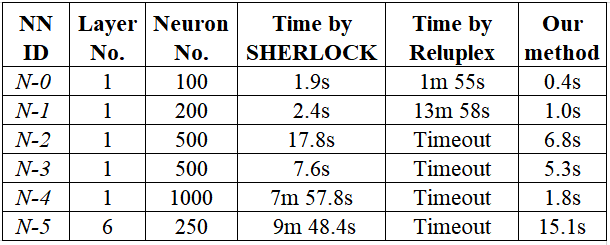
\includegraphics[width=0.9\linewidth]{images/robustnessVerification/f2.png}
% 	\caption{Comparison with SHERLOCK and Reluplex}
% 	\label{fig-2}
% \end{figure}

% \begin{figure*}[ht]
% 	\begin{minipage}{0.46\linewidth}
% 	\centering
% 	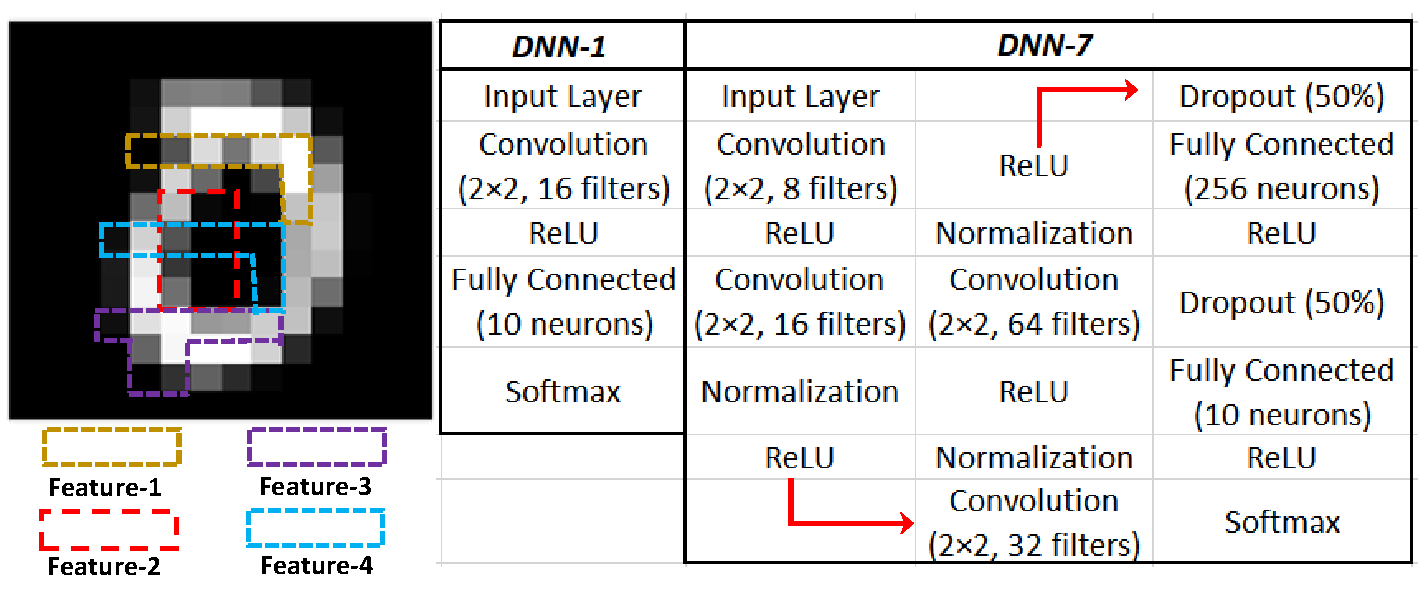
\includegraphics[width=1\linewidth]{images/robustnessVerification/f4.pdf}
% 	\subcaption{}
% 		\end{minipage}
% 		\begin{minipage}{0.54\linewidth}
% 		\centering
% 	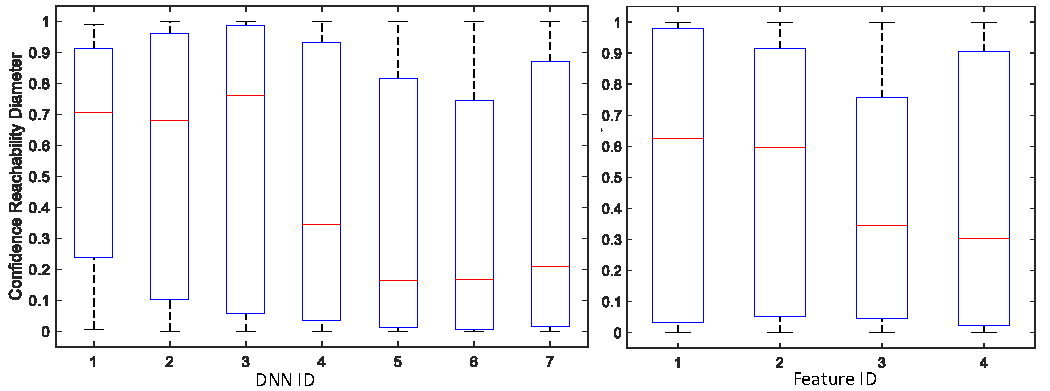
\includegraphics[width=1\linewidth]{images/robustnessVerification/f8.pdf}
% 		\subcaption{}
% 		\end{minipage}
% 			\vspace{-1pt}
% 			\caption{(a) The four features and the architecture of DNN-1 and DNN-7. (b) Left: boxplots of confidence reachability diameters for 7 DNNs, based on $4\times20$ analyses of each DNN. Right: boxplot of confidence reachability diameters for 4 features, based on $7\times20$ analyses of each feature. The red line represents the median value: a lower value indicates a more robust model or feature.}
% 	\label{fig-3}
% \end{figure*}

% \begin{figure*}[t]
% 	\begin{minipage}{0.32\linewidth}
% 	\centering
% 	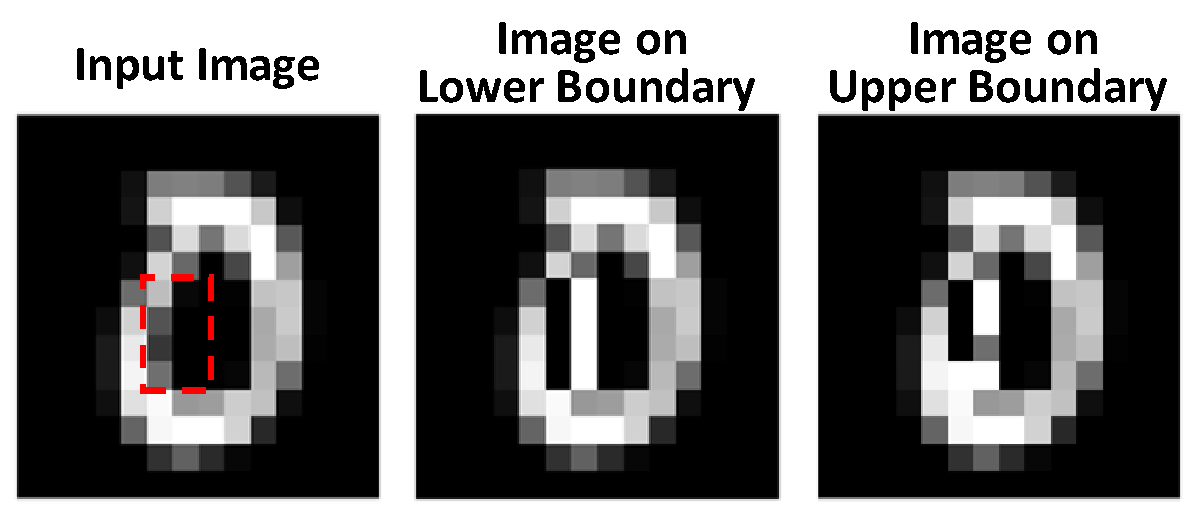
\includegraphics[width=0.9\linewidth]{images/robustnessVerification/f3.pdf}
% 		\subcaption{}
% 	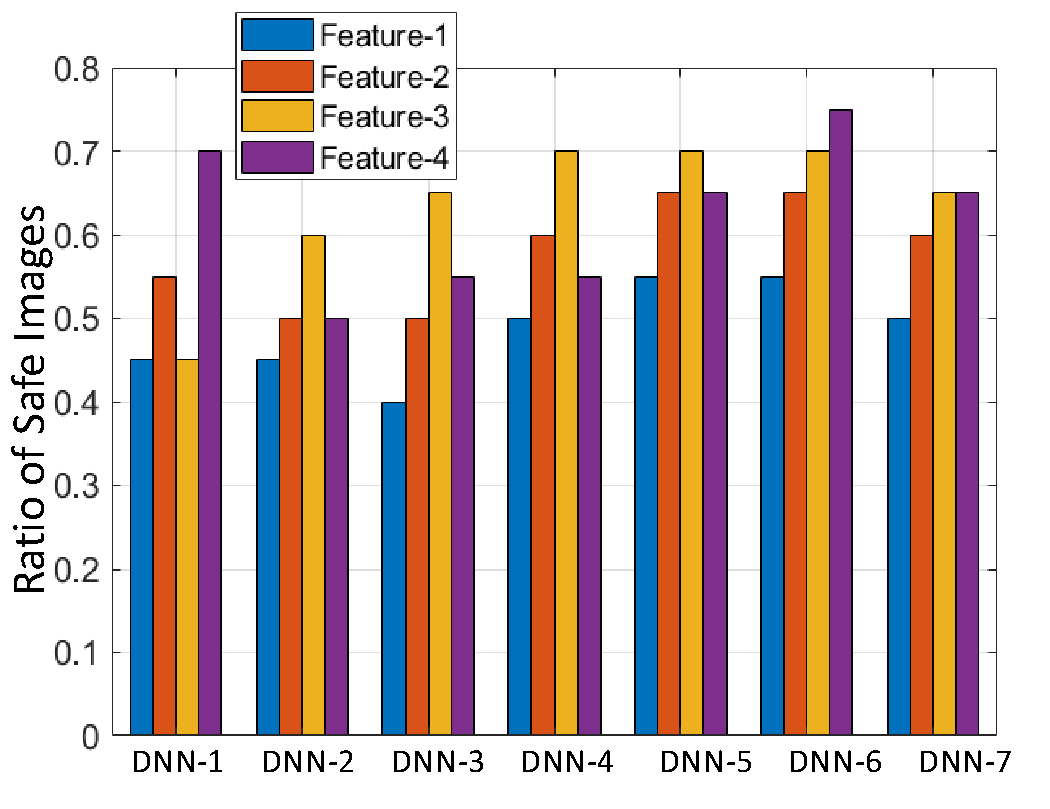
\includegraphics[width=1\linewidth]{images/robustnessVerification/f6.pdf}
% 	\subcaption{}
% 		\end{minipage}
% 		\begin{minipage}{0.68\linewidth}
% 		\centering
% 	\centering
% 	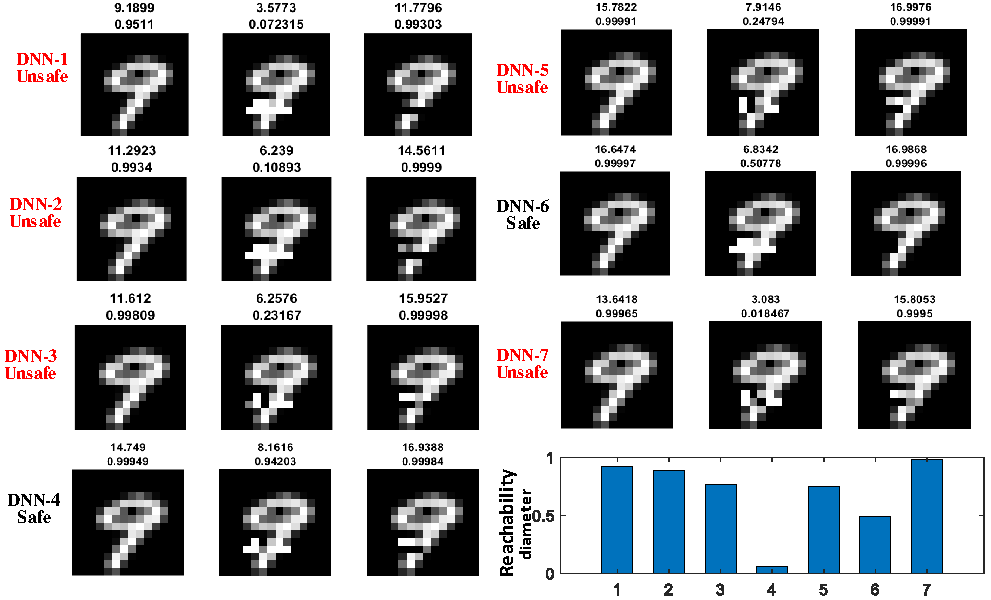
\includegraphics[width=1\linewidth]{images/robustnessVerification/f7.pdf}
% 	\subcaption{}
% 		\end{minipage}
% 			\caption{(a) Left: an original image (logit is 11.806, confidence of output being `0' is 99.95\%), where area marked by dashed line is the feature. Middle: an image on the confidence lower bound. Right: an image on the confidence upper bound; for the output label `0', the feature's output range is $[74.36\%,99.98\%]$, and logit reachability is $[7.007, 13.403]$. (b) Ratios of safe images for 7 DNNs and 4 features. (c) A detailed example comparing the safety and robustness of DNNs for image '9' and Feature-3: the top number in the caption of each figure is logit and the bottom one is confidence; the unsafe cases are all misclassified as `8'; the last bar chart shows their confidence reachability diameters.}
% 	\label{fig-4}
% \end{figure*}
 

% \subsection{Case Study One: Safety Verification}

% We use our tool to conduct logit and output range analysis.
% %for verifying the safety of deep neural networks, and compare robustness of different networks and input subspaces. 
% Seven convolutional neural networks, represented as DNN-1,...,DNN-7, were trained on the MNIST dataset. Images are resized into $14\times 14$ to enforce that a DNN with deeper layers tends to over-fit. The networks have different layer types, including ReLu, dropout and normalization, and the number of layers ranges from $5$ to $19$. Testing accuracies range from $95\%$ to $99\%$, and $\epsilon=0.05$ is used in our experiments.

% We randomly choose 20 images (2 images per label) and manually choose 4 features
% %\footnote{We also conduct experiments in which features are selected by object detection techniques such as SIFT \cite{Lowe1999}. We cannot include the results for space limit, but the conclusions are similar. } 
% such that each feature contains 8 pixels, i.e., $X'=[0,1]^8$. Fig.~\ref{fig-3} (a) illustrates the four features and the architecture of two DNNs with the shallowest and deepest layers, \ie~DNN-1 and DNN-7. 

% \vspace{1mm}

% \noindent{\bf Safety Verification}
% %
% %Then we conduct the reachability analysis for those features. 
% Fig.~\ref{fig-4} (a) shows an example: for DNN-1, Feature-4 is \emph{guaranteed to be safe} with respect to the image $x$ and the input subspace $X'$.
% %to any adversarial perturbation. 
% Specifically, the reachability interval is $R(\Pi_0,X',\epsilon) = [74.36\%,99.98\%]$, which means that $l(\Pi_0,X',\epsilon)=74.36\%$. By this, we have $u(\oplus_{-0},X',\epsilon) \leq (1-0.7436) < 0.7436 = l(\Pi_0,X',\epsilon)$. Then, by Theorem \ref{thm:safety}, we have 
% $\Safe(\text{DNN-1},x,X')$. Intuitively, no matter how we manipulate this feature, the worst case is to reduce the confidence of output being `0' from 99.95\% (its original confidence probability) to 74.36\%. 


% \subsection{Case Study Two: Statistical Quantification of Robustness}


% \noindent{\bf Statistical Comparison of Safety}
% %
% Fig.~\ref{fig-4} (b) compares the ratios of safe images for different DNNs and features. It shows that: \one~no DNN is 100\% safe on those features: DNN-6 is the safest one and DNN-1, DNN-2 and DNN-3 are less safe, which means a DNN with well chosen layers are safer than those DNNs with very shallow or deeper layers; and \two~the safety performance of different DNNs is consistent for the same feature, which suggests that the feature matters -- some features are easily perturbed to yield adversarial examples, e.g., Feature-1 and Feature-2.

% \vspace{1mm}

% \noindent{\bf Statistical Comparison of Robustness}
% %
% Fig.~\ref{fig-3} (b) compares the robustness of networks and features with two boxplots over the reachability diameters, where the function $o$ is $\Pi_j$ for a suitable $j$. We can see that DNN-6 and DNN-5 are the two most robust, while DNN-1, DNN-2 and DNN-3 are less robust. Moreover, Feature-1 and Feature-2 are less robust than Feature-3 and Feature-4. 

% %Together with the above, we can see that 
% We have thus demonstrated that
% reachability analysis with our tool can be used to quantify the safety and robustness of deep learning models. In the following, we perform a comparison of networks over a fixed feature. 

% \vspace{1mm}

\subsection{A Running Numerical Example}

In this section, we will use a numerical example to illustrate the fundamental differences between the reachability analysis method, DeepGO, constraint-solver based approach~\cite{bunel2017piecewise,CNR2017,ehlers2017formal1}, and $AI^2$ - a verification method based Abstract Interpretation (AI)~\cite{gehr2018ai21}.

Fig.~\ref{fig-E2} shows the details of a neural network we used for investigation. This toy neural network has two input $x_1$ and $x_2$, two output $y_1$ and $y_2$. It contains one hidden layer with ReLU activation functions. We denote the ReLU activation by two parts: one part is $r_1$ and $r_1$ denoting the values before the activation, another part is $h_1$ and $h_2$ representing the values after activation. In this numerical example, we aim to solve the following reachability problem.

\begin{problem}\label{problem-E1}
{\em Given a neural network and the box-constraints on its inputs, i.e., $x_1\in [4,6], x_2 \in [4.5,5]$, what is the output range of $y_1$?}
\end{problem}

We will first show constraint-solver based solution, then reveal how $AI^2$ works and finally show how to use DeepGO to solve this problem.
 
\begin{figure}[t]
	\centering
	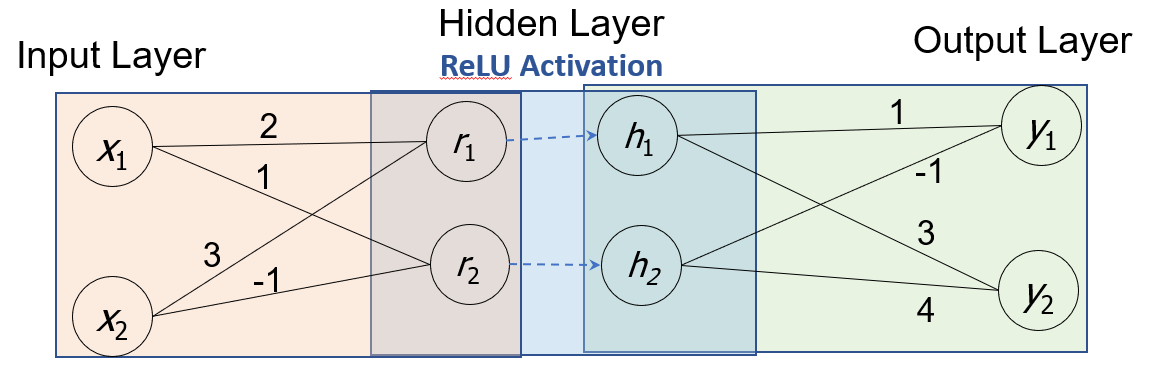
\includegraphics[width=0.85\linewidth]{images/robustnessVerification/Capture5.PNG}
	\caption{Encoding the whole neural network layer by layer on a neural networks with one ReLU-based hidden layer}
	\label{fig-E2}
\end{figure}
  
\subsubsection{Constraint-Solver based Approach}

As discussed in previous chapters, the majority of the solutions to solve Problem~\ref{problem-E1} are based on MILP or LP solvers, including SHERLOCK~\cite{dutta2017output}, Reluplex~\cite{katz2017reluplex}, Planet~\cite{ehlers2017formal1}, MIP~\cite{CNR2017} and BaB~\cite{bunel2017piecewise}, etc. We will reveal the basic idea of those works by using an LP-based solver as an example.

The first step is to encode the input and neural networks. As shown in Fig.~\ref{fig-E2}, we can encode the whole neural network layer by layer.

\begin{equation}\label{eqn-encode}
    \begin{split}
        \begin{cases}
        r_1 = 2x_1 + 3x_2\\
        r_2 = x_1 - x_2\\
        h_1 = \begin{cases}
    r_1, & \text{if $r_1\geq 0$}.\\
    0, & \text{otherwise}.
  \end{cases}\\
  h_2 = \begin{cases}
    r_2, & \text{if $r_2\geq 0$}.\\
    0, & \text{otherwise}.
  \end{cases}\\
  y_1 = h_1 - h_2\\
  y_2 = 3h_1 - 4h_2\\
  4 \leq x_1 \leq 6\\
  4.5 \leq x_2 \leq 5
  \end{cases}
    \end{split}
\end{equation}

Then, to estimate the reachable interval of $y_1$, we also need to incorporate the target problem and formulate them into {\em four} linear programming problems based on the activation patterns of hidden neurons, as shown by the below equation.

\begin{equation}\label{eqn-encode}
    \begin{split}
       & \begin{cases}
        \max/\min~~y_1 = x_1 +4x_2\\
        \text{s.t.} \quad  2x_1 + 3x_2\geq 0\\
        \qquad x_1 - x_2 \geq 0\\
        \qquad 4\leq x_1 \leq 6\\
        \qquad 4.5\leq x_1 \leq 5\\
  \end{cases} 
  \bigcup  
        \begin{cases}
        \max/\min~~y_1 = 2x_1 +3x_2\\
        \text{s.t.} \quad  2x_1 + 3x_2\geq 0\\
        \qquad x_1 - x_2 \leq 0\\
        \qquad 4\leq x_1 \leq 6\\
        \qquad 4.5\leq x_1 \leq 5\\
  \end{cases}\\
  \bigcup &
  \begin{cases}
        \max/\min~~y_1 = -x_1 +x_2\\
        \text{s.t.} \quad  2x_1 + 3x_2\leq 0\\
        \qquad x_1 - x_2 \geq 0\\
        \qquad 4\leq x_1 \leq 6\\
        \qquad 4.5\leq x_1 \leq 5\\
  \end{cases}
    \bigcup
  \begin{cases}
        \max/\min~~y_1 = 0\\
        \text{s.t.} \quad  2x_1 + 3x_2\leq 0\\
        \qquad x_1 - x_2 \leq 0\\
        \qquad 4\leq x_1 \leq 6\\
        \qquad 4.5\leq x_1 \leq 5\\
  \end{cases}
    \end{split}
\end{equation}

By solving the above four linear programming problems using an LP solver, we can solve Problem~\ref{problem-E1} and calculate its reachable confidence interval $[21.5, 26]$.

\subsubsection{Abstract Interpretation based Approach}

A well-established verification work using Abstract Interpretation is $AI^2$~\cite{gehr2018ai21}. It phrases the problem of certifying neural networks in the classic abstract interpretation framework. The key ingredient in $AI^2$ is the layer-by-layer over-approximation of the neural network using zonotope-based abstract interpretation. 

Fig.~\ref{fig-E11} depicts the procedure of layer-by-layer zonotope abstract interpretation in $AI^2$ for solving Problem~\ref{problem-E1}. $AI^2$ first adopts a zonotope to abstract all the inputs. 
%
\begin{equation}
    \begin{split}
        \mathbf{Z}_1 = \{(x_1,x_2)~|~x_1 = a_1 +5; x_2= 0.25a_2 +4.75\}
    \end{split}
\end{equation}
%
where $a_1 \in [-1,1]$ and $a_2 \in [-1,1]$.

Then it performs the zonotope abstract transformation based on the affine transformation from the input layer into the pre-activation layer. Please note that affine transformation is exact in zonotope-based abstraction.
%
\begin{equation}
    \begin{split}
        \mathbf{Z}_2 = \{(r_1,r_2)~|~r_1 = 24.25+2a_1+0.75a_2; r_2= 0.25 + a_1 - 0.25a_2\}
    \end{split}
\end{equation}
%
where $a_1 \in [-1,1]$ and $a_2 \in [-1,1]$.


\begin{figure}[t]
	\centering
	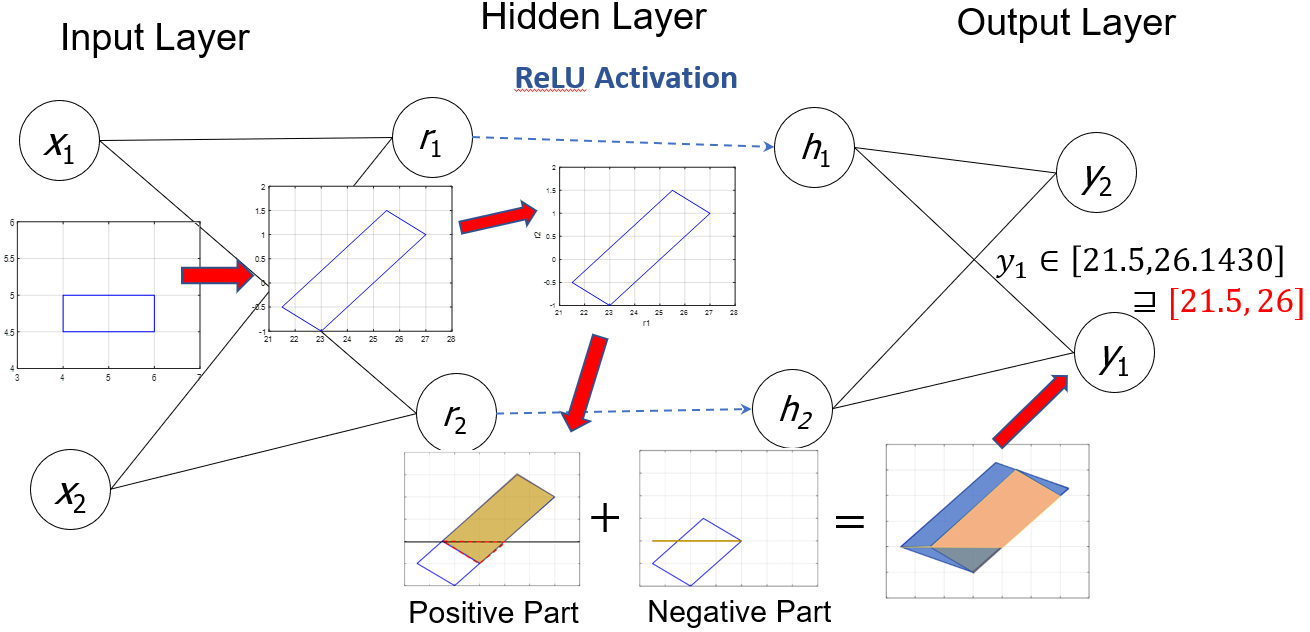
\includegraphics[width=1\linewidth]{images/robustnessVerification/Capture8.PNG}
	\caption{Illustration of layer-by-layer over-approximation using zonotope abstract interpretation in $AI^2$}
	\label{fig-E11}
\end{figure}

Next, $AI^2$ considers the zonotope over-approximation on the first ReLU hidden neuron. Since $r_1\geq 0$ always holds, zonohedron $\mathbf{Z}_2$ will transfer into the next layer without over-approximation loss. Thus we have $\mathbf{Z}_3 = \mathbf{Z}_2$. However, for the second ReLU hidden neuron, the zonotope abstraction is complicated since $r_2$ is partially negative and partially positive, which requires two cases:

\begin{itemize}
    \item Zonotope Over-approximation on Positive Part: As shown in Figure~\ref{fig-E11}, the positive part $\mathbf{Z}_3\cap \{r_2\geq 0\}$ is not a zonohedron. So we perform the zonotope over-approximation and get a new zonohedron:
    $$\mathbf{Z}_{4,p} = \{(h_1,h_2)~|~h_1 = 24.75+1.5a_1+0.75a_2; h_2= 0.5 + 0.75a_1 - 0.25a_2\}$$
    
     \item Zonotope Over-approximation on Negative Part: Similarly, we get a new zonotope 
    $$\mathbf{Z}_{4,n} = \{(h_1,h_2)~|~h_1 = 23.25+0.75a_1+a_2; r_2 = 0\}$$
\end{itemize}

Then, as shown in Fig.~\ref{fig-E11}, we perform a joint on two zonotopes $\mathbf{Z}_{4,p}\cup \mathbf{Z}_{4,n}$, and perform another zonotope over-approximation:
%
\begin{equation}
    \mathbf{Z}_5 = \{(h_1,h_2)~|~h_1 = 24.3929+1.6429a_1+1.25a_2; h_2= 0.5714 + 0.8214a_1 - 0.25a_2\}
\end{equation}
%
where $a_1 \in [-1,1]$ and $a_2 \in [-1,1]$.


Finally, we can get the symbolic express on $y_1$ based on the affine transformation from after-activation layer to output layer:
\begin{equation}
    y_1 = h1 - h2 = 23.8215 + 0.8215a_1 - 1.5a_2
\end{equation}
where $a_1 \in [-1,1]$ and $a_2 \in [-1,1]$. Thus, using $AI^2$, we can get the reachable output of $y_1$ is $[21.5, 26.1430] \supseteq	[21.5, 26]$, which is an over-approximation of the actual reachable state of the neural network. As illustrated by Fig.~\ref{fig-E12}, the yellow area is the actual information passed into the output layer, and the blue area is the over-approximation loss brought by the layer-by-layer zonotope abstractions.

\begin{figure}[t]
	\centering
	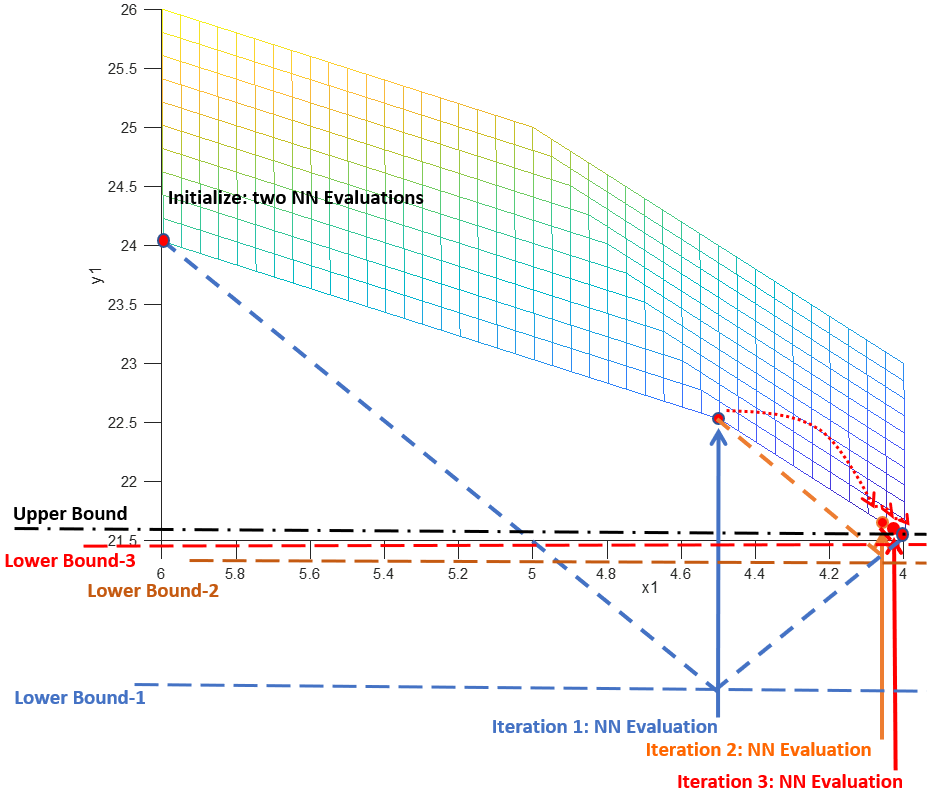
\includegraphics[width=0.9\linewidth]{images/robustnessVerification/Capture10.PNG}
	\caption{Illustration of working mechanism of DeepGO for solving the reachability problem}
	\label{fig-E13}
\end{figure}
  

\subsubsection{Reachability Analysis by DeepGO}


Now we show how DeepGO solve this reachability problem. As we can prove the target neural network in Fig.~\ref{fig-1} is proved to be Lipschitz continuous~\cite{szegedy2014intriguing,RHK2018}, to solve Problem~\ref{problem-E1}, it can be reduced to solve the following minimisation problems.
\begin{equation}\label{eqn-deepagn}
   \begin{cases}
        \min_{x_1,x_2}~~y_1 = f(x_1,x_2)\\
        \text{s.t.} \quad 4\leq x_1 \leq 6\\
        \qquad 4.5\leq x_1 \leq 5\\
  \end{cases}
\end{equation}

By solving the above two problems, we can get the reachable value of $y_1$. Fig.~\ref{fig-E13} illustrates the optimisation procedure of DeepGO iteration by iteration\footnote{For visualisation, we just show the $x_1$ dimension.}.

\begin{itemize}
    \item Initialisation: It evaluates two ending points on $x_1$: 4 and 6, and gets the Upper Bound-1 and Lower Bound-1.
    \item Iterations: DeepGO then evaluates $y_1$ on the point of Lower Bound-1, and refines the lower bound to get Lower Bound-2 (described in Section~\ref{sec:onedimensional}). Similarly, we continue the optimisation iterations and get a series of lower bounds.
    \item Termination: After the gap between lower bound and upper bound is close enough, i.e., smaller than a positive number $\epsilon = 0.0001$, we stop and return the value of $y_1^* = 21.5$, which is the lowest value that the neural network can reach in Problem~\ref{problem-E1}.
\end{itemize}

To get the largest reachable value, We replace objective function in Eqn.~\ref{eqn-deepagn} by $y_1 = - f(x_1,x_2)$ and perform the same procedure to get $y_1^{**} = 26$. By DeepGO, we can finally get the reachable interval of the neural network: $y_1 = [21.5, 26]$. 

\begin{figure}[t]
	\centering
	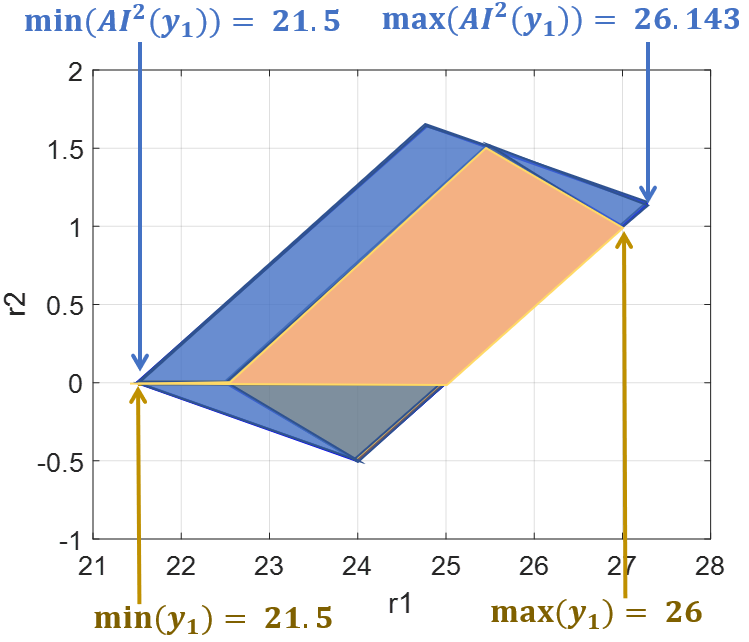
\includegraphics[width=0.55\linewidth]{images/robustnessVerification/Capture9.PNG}
	\caption{The comparison between $AI^2$ and DeepGO in terms of over-approximation error}
	\label{fig-E12}
\end{figure}

In summary, for Problem~\ref{problem-E1}, as we can see from Fig.~\ref{fig-E12}, DeepGO can calculate the reachable range of the neural network without an over-approximation error, but $AI^2$ brings a non-trivial error due to its over-approximation nature from the abstract interpretation. On the other hand, although LP/MILP based solution can also obtain an exact reachable range, DeepGO is much more efficient, especially for a neural network with a massive number of neurons.

%\subsection{Conclusion}

%This chapter introduces a reachability analysis method for deep neural networks, called DeepGO. It has provable guarantees and can be applied to neural networks with deep layers and nonlinear activation functions. The numerical example demonstrates the merits of this approach, which marks an important step towards a practical, guaranteed safety verification for DNNs.

